\chapter{Results and Discussion}
\section{Introduction}
We have discussed the implementation of CrazyOS. However, discussing the implementations is not enough for the reader needs to get their hands dirty to understand this project. For this reason, in this chapter we will present the results of this project. These results are obtained by running the operating system in QEMU's emulation of a system based on i386 processor. We have discussed how various commands are used in the shell and present to the reader the only three known bugs known in the operating system at the time of writing of this report.

\section{Cloning \& Running CrazyOS}
Since its inception, CrazyOS's version control has been done using Git and the repository has been hosted on Github. To download the source files of the project on a local machine, the user must first install Git and generate SSH keys and link them with his account on Github. Once these preliminary tasks have been done, the user has to type the following command in a terminal to clone CrazyOS:
\begin{Verbatim}
$ git clone git@github.com:PraneetKapoor2619/CrazyOS.git
\end{Verbatim} 
The \$ should be ignored; it is just a standard way of telling readers that they should type the text ahead in a terminal.\\
Once the project has been cloned, the reader has to make sure that the version of CrazyOS that he uses has the short commit ID 1a17fa0. For this, the following command has to be entered in the terminal:
\begin{Verbatim}
$ git reset --hard 1a17fa0
\end{Verbatim}
To move to the project directory, the following command is executed:
\begin{Verbatim}
$ cd CrazyOS/8086/
\end{Verbatim}
Once in the project directory, the user must create a build directory by the following command:
\begin{Verbatim}
$ mkdir build
\end{Verbatim}
The binary files and the disk images are built using \texttt{make build} command. To run the operating system, type
\begin{Verbatim}
$ make run
\end{Verbatim}
To exit QEMU without powering off the emulator from CrazyOS's shell, just press \texttt{Ctrl + Alt + Q}. \texttt{build} directory is cleaned by using \texttt{make clean} command. To remove \texttt{asm.bin} and \texttt{disk2.bin} in the \texttt{build} directory, the following commands should be used:
\begin{Verbatim}
$ rm build/asm.bin build/disk2.bin
\end{Verbatim}

\section{Using the Shell}
Upon running the emulation, the user will be greeted with a startup screen showing a text message, and current time and date, as shown in \autoref{fig:startupscrn}).
\begin{figure}[H]
  \centering
  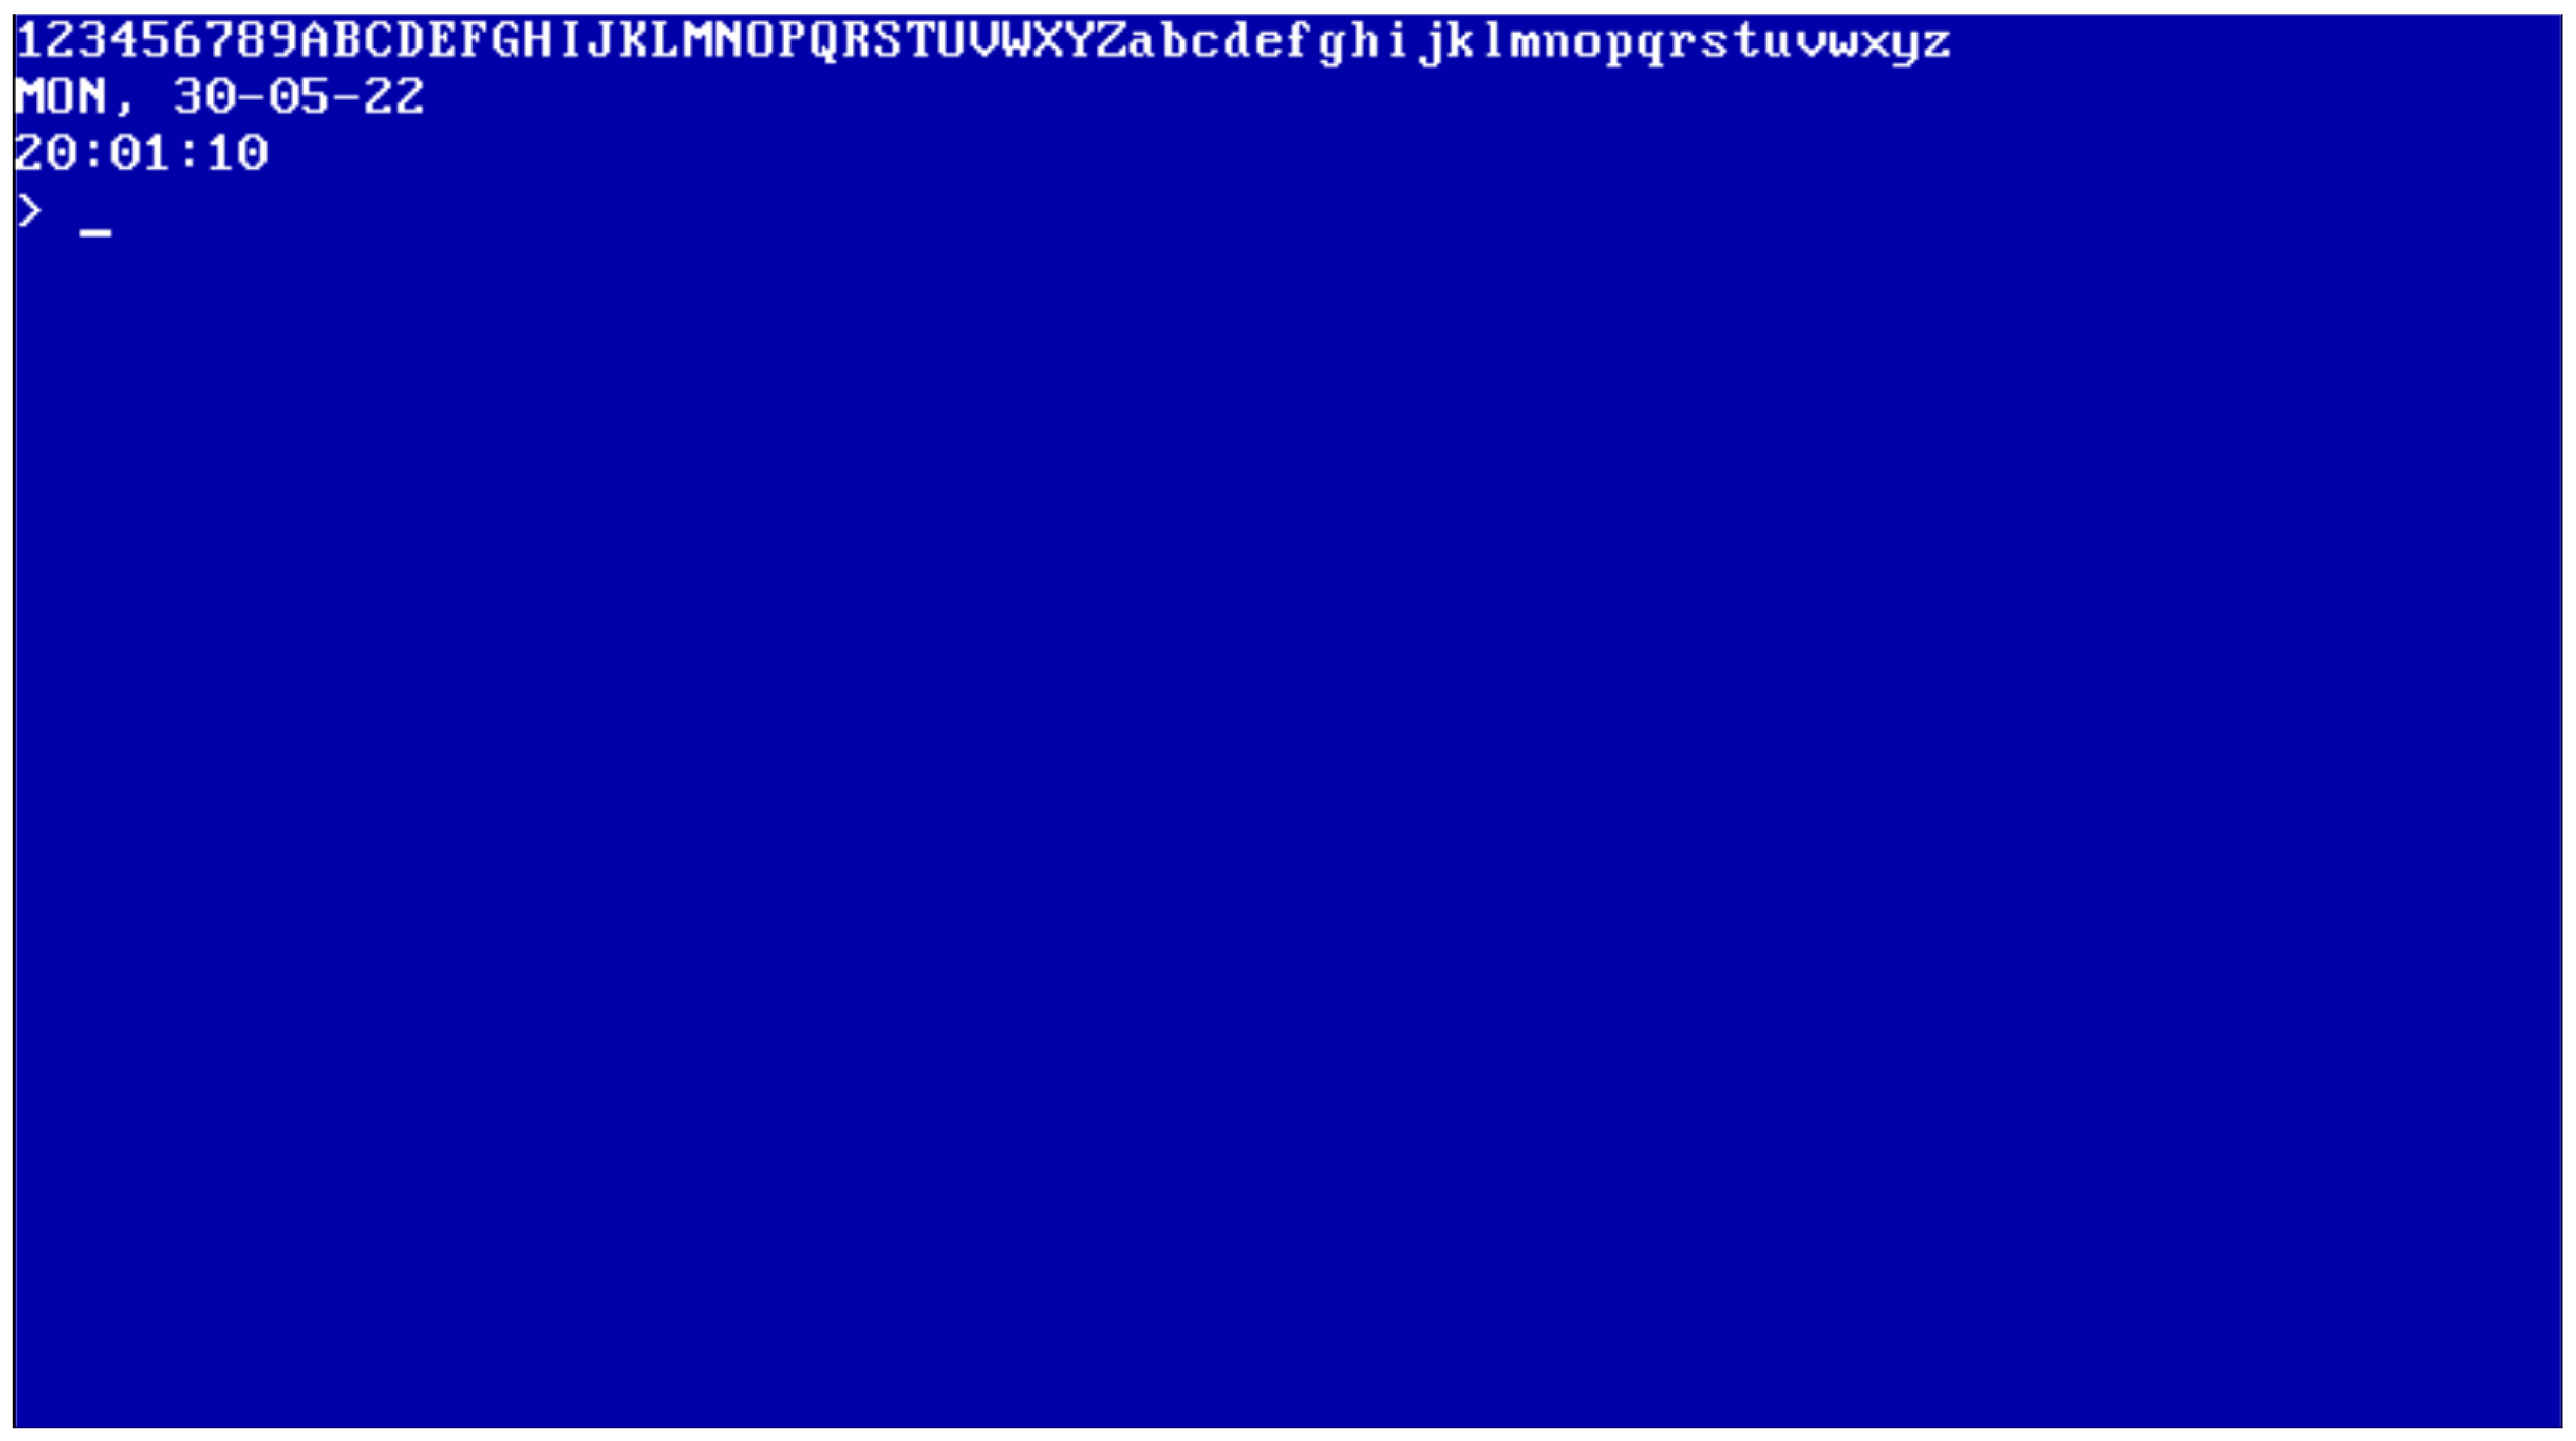
\includegraphics[scale=0.25]{figures/startupscrn.eps}
  \caption{CrazyOS startup screen}
\label{fig:startupscrn}
\end{figure}

\subsection{Using time, date, srng, and clear}
Using \texttt{time} and \texttt{date} command the user can know the current time and date, respectively. By typing \texttt{srng} multiple times, the user can generate different pseudo-random numbers. To clear the screen, \texttt{clear} command is used. Output of these commands are shown in \autoref{fig:timedatesrng}.
\begin{figure}[H]
  \begin{subfigure}{.5\textwidth}
  \centering
  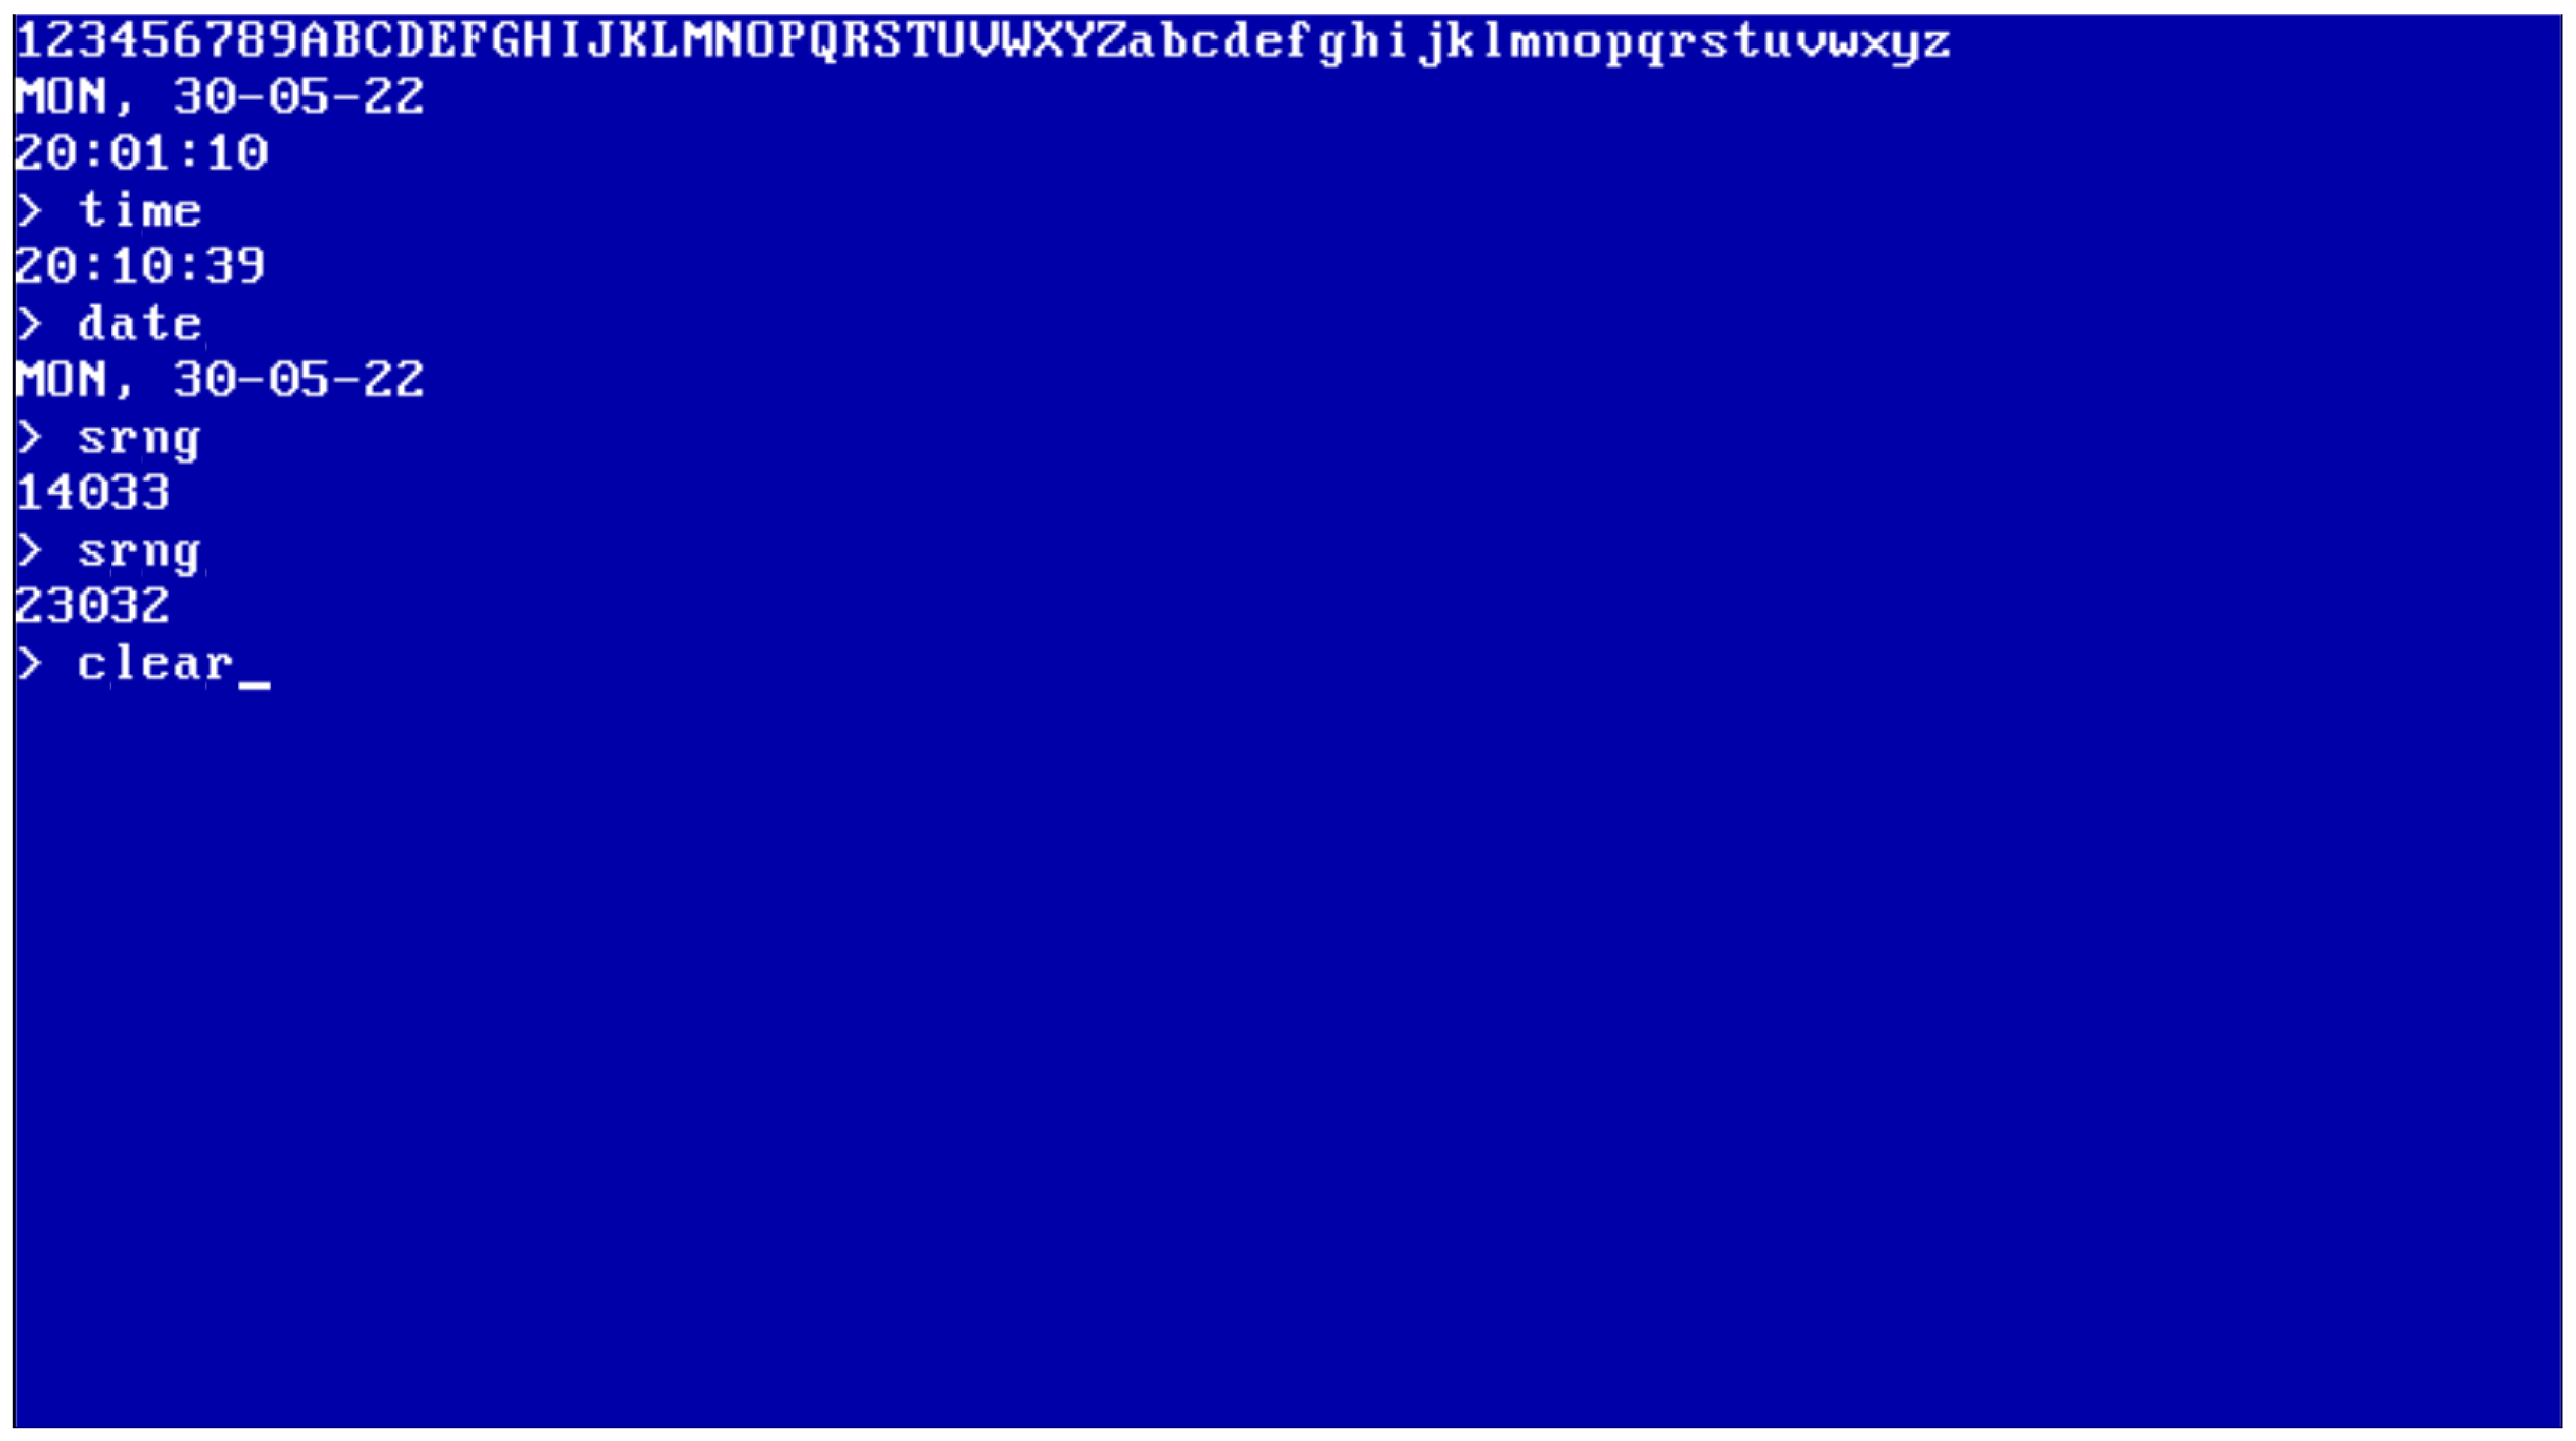
\includegraphics[scale=0.13]{figures/timedatesrng.eps}
  \caption{Using \texttt{time}, \texttt{date}, and \texttt{srng} commands}
  \end{subfigure}
  \begin{subfigure}{.5\textwidth}
  \centering
  
\includegraphics[scale=0.13]{figures/cleareffect.eps}
  \caption{Effect of \texttt{clear} command}
  \end{subfigure}
\caption{Using \texttt{time}, \texttt{date}, \texttt{srng}, and \texttt{clear} commands}
\label{fig:timedatesrng}
\end{figure}

\subsection{Running Disk Applications}
The binary of \texttt{../disk-apps/soundnlight.asm} is loaded at the first sector of \texttt{disk2.bin}. The application is first read using \texttt{disk read} command. In \autoref{fig:dskrdrun}, we have loaded the application in the 5th block. To run it, we type \texttt{run 5000:0000}. This performs an intersegment call and runs the application, thus producing coloured pixels and notes corresponding to the byte of the kernel that is being read, as shown in \autoref{fig:soundnlight}. As this application has no far return instruction, \texttt{retf}, we need to kill the emulation using \texttt{Ctrl + Alt + Q} key combo.
\begin{figure}[H]
  \begin{subfigure}{.5\textwidth}
  \centering
  
\includegraphics[scale=0.13]{figures/dskrdrun.eps}
  \caption{Using \texttt{disk read} and \texttt{run}}
  \label{fig:dskrdrun}
  \end{subfigure}
  \begin{subfigure}{.5\textwidth}
  \centering
  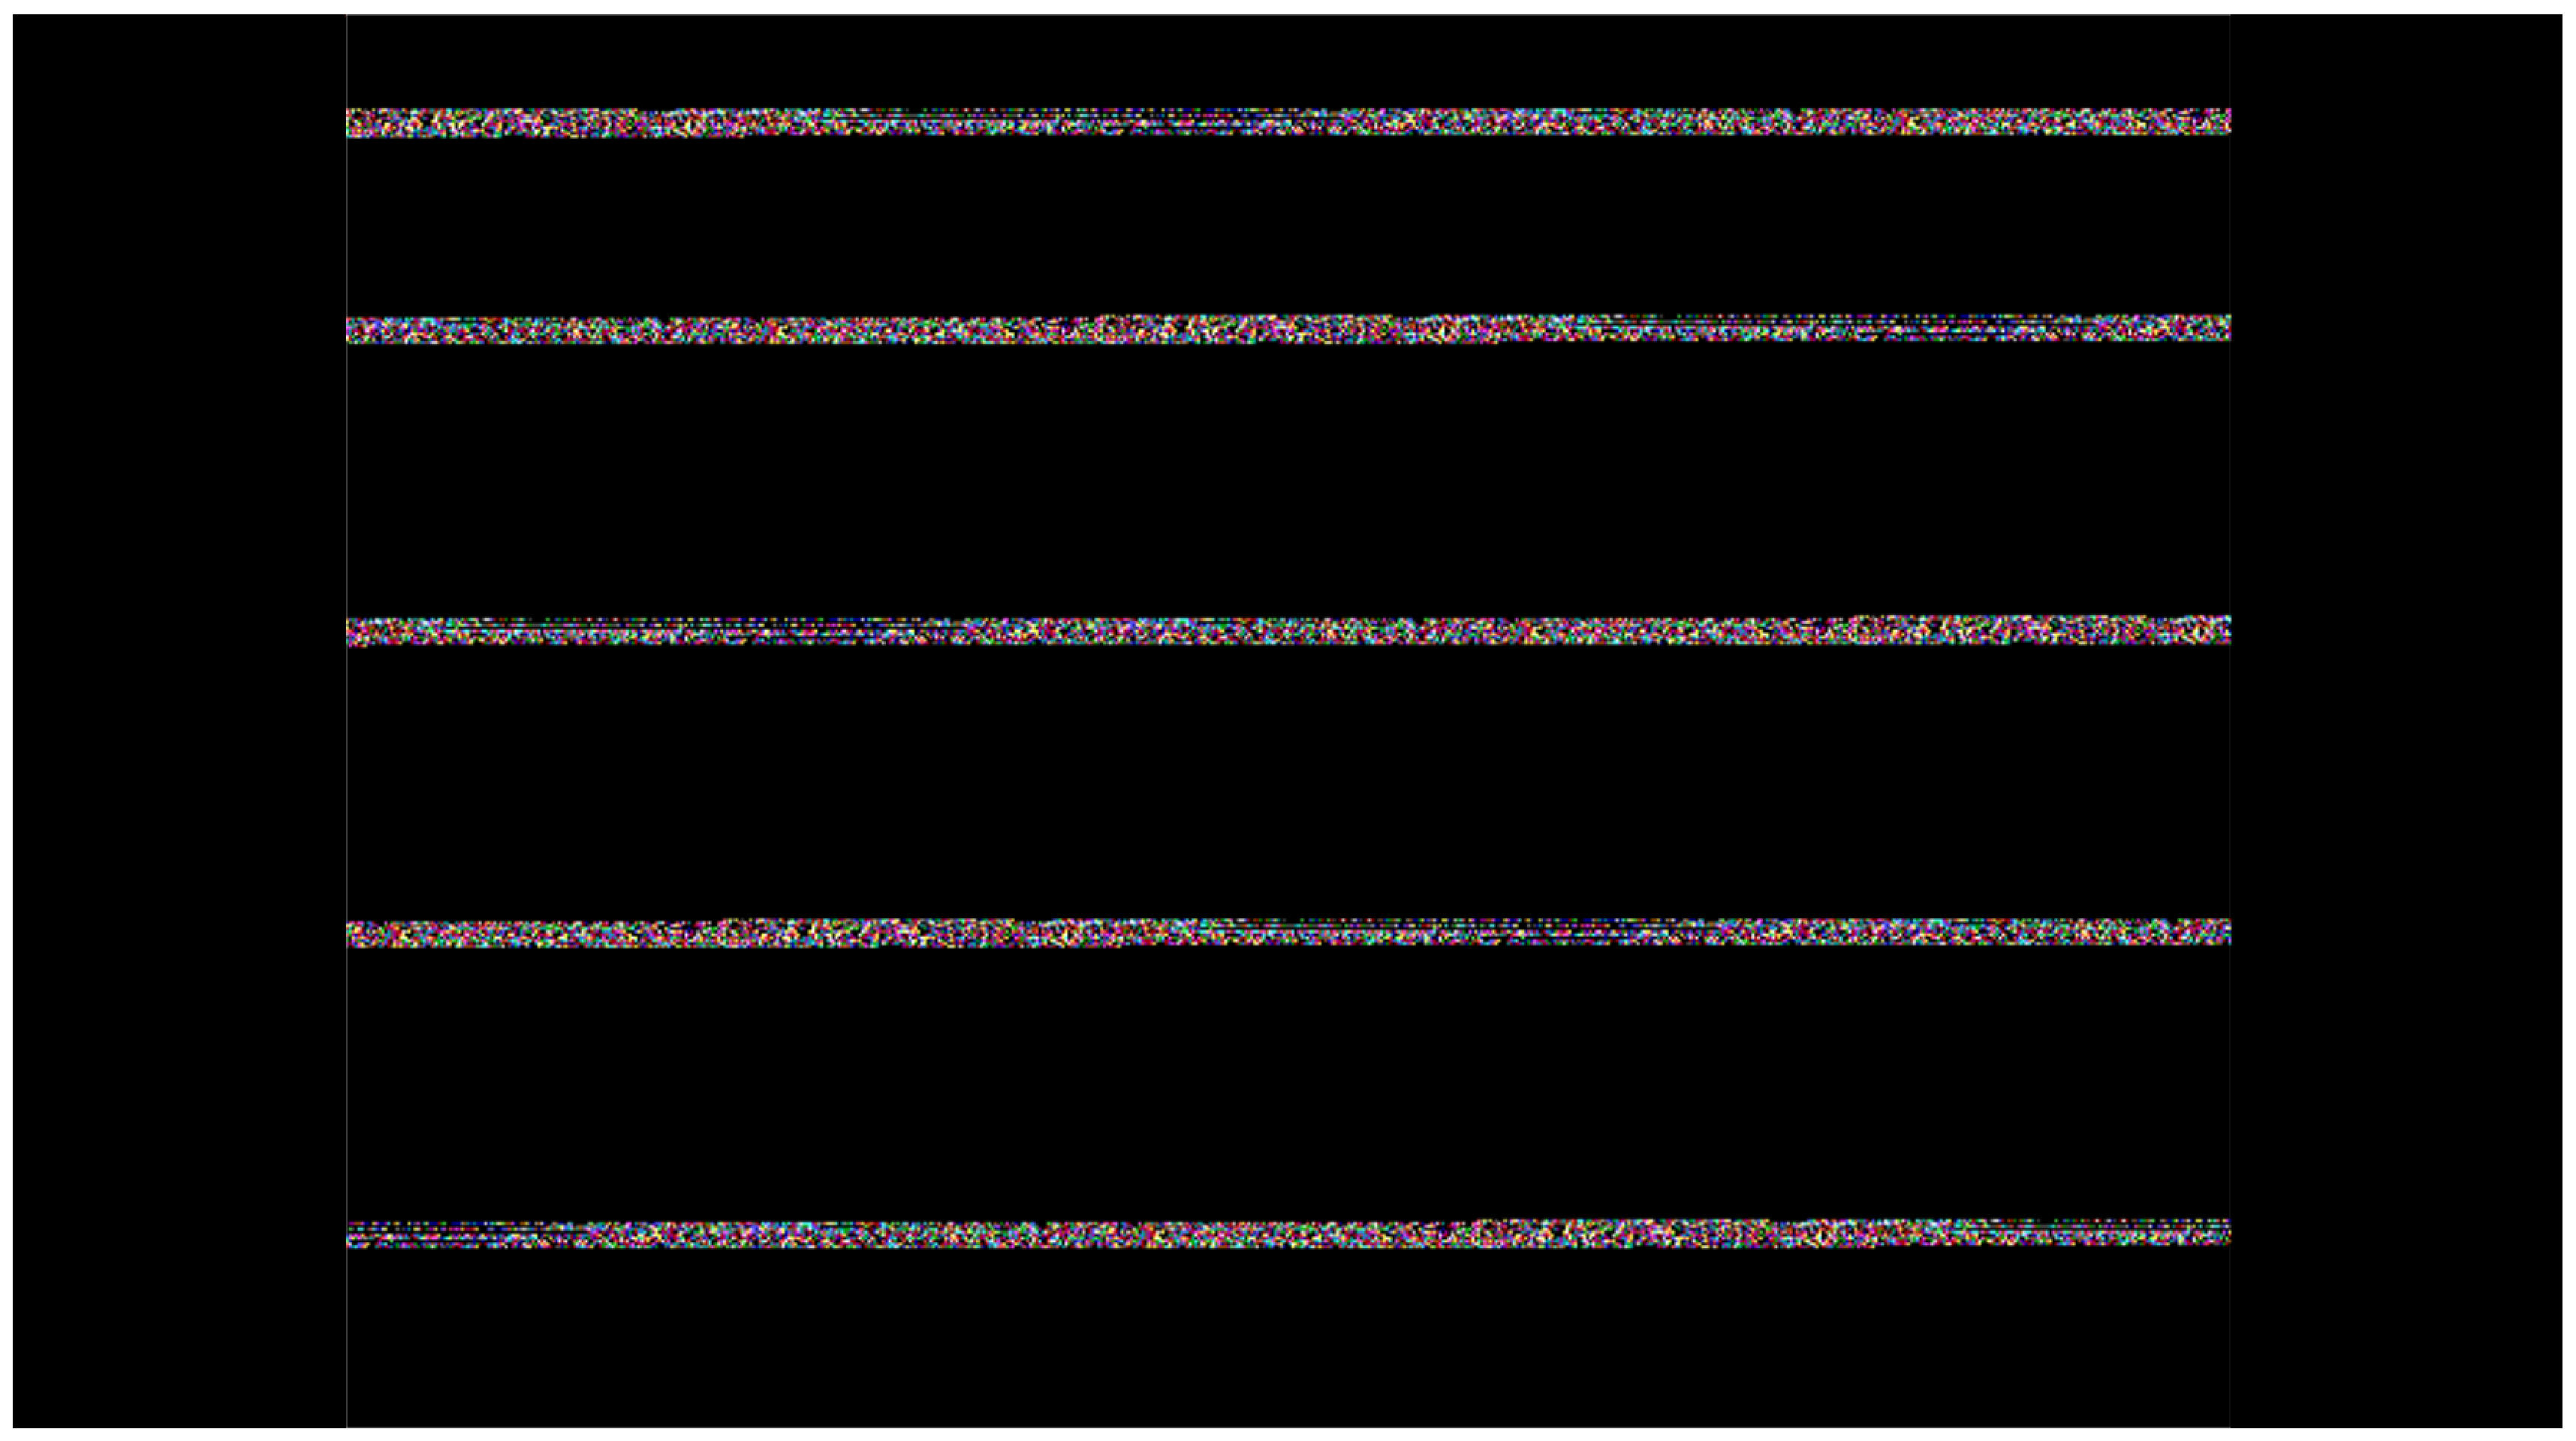
\includegraphics[scale=0.13]{figures/soundnlight.eps}
  \caption{Running \texttt{soundnlight}}
  \label{fig:soundnlight}  
  \end{subfigure}
\caption{Using \texttt{disk read} and \texttt{run} commands to run a disk application}
\end{figure}

\subsection{Power Commands}
\texttt{power} command is used to manage power of the machine using APM. Its use is shown in \autoref{fig:powercom}. Note that the command \texttt{power level} prints \texttt{Power level unknown}.
\begin{figure}[H]
  \centering
  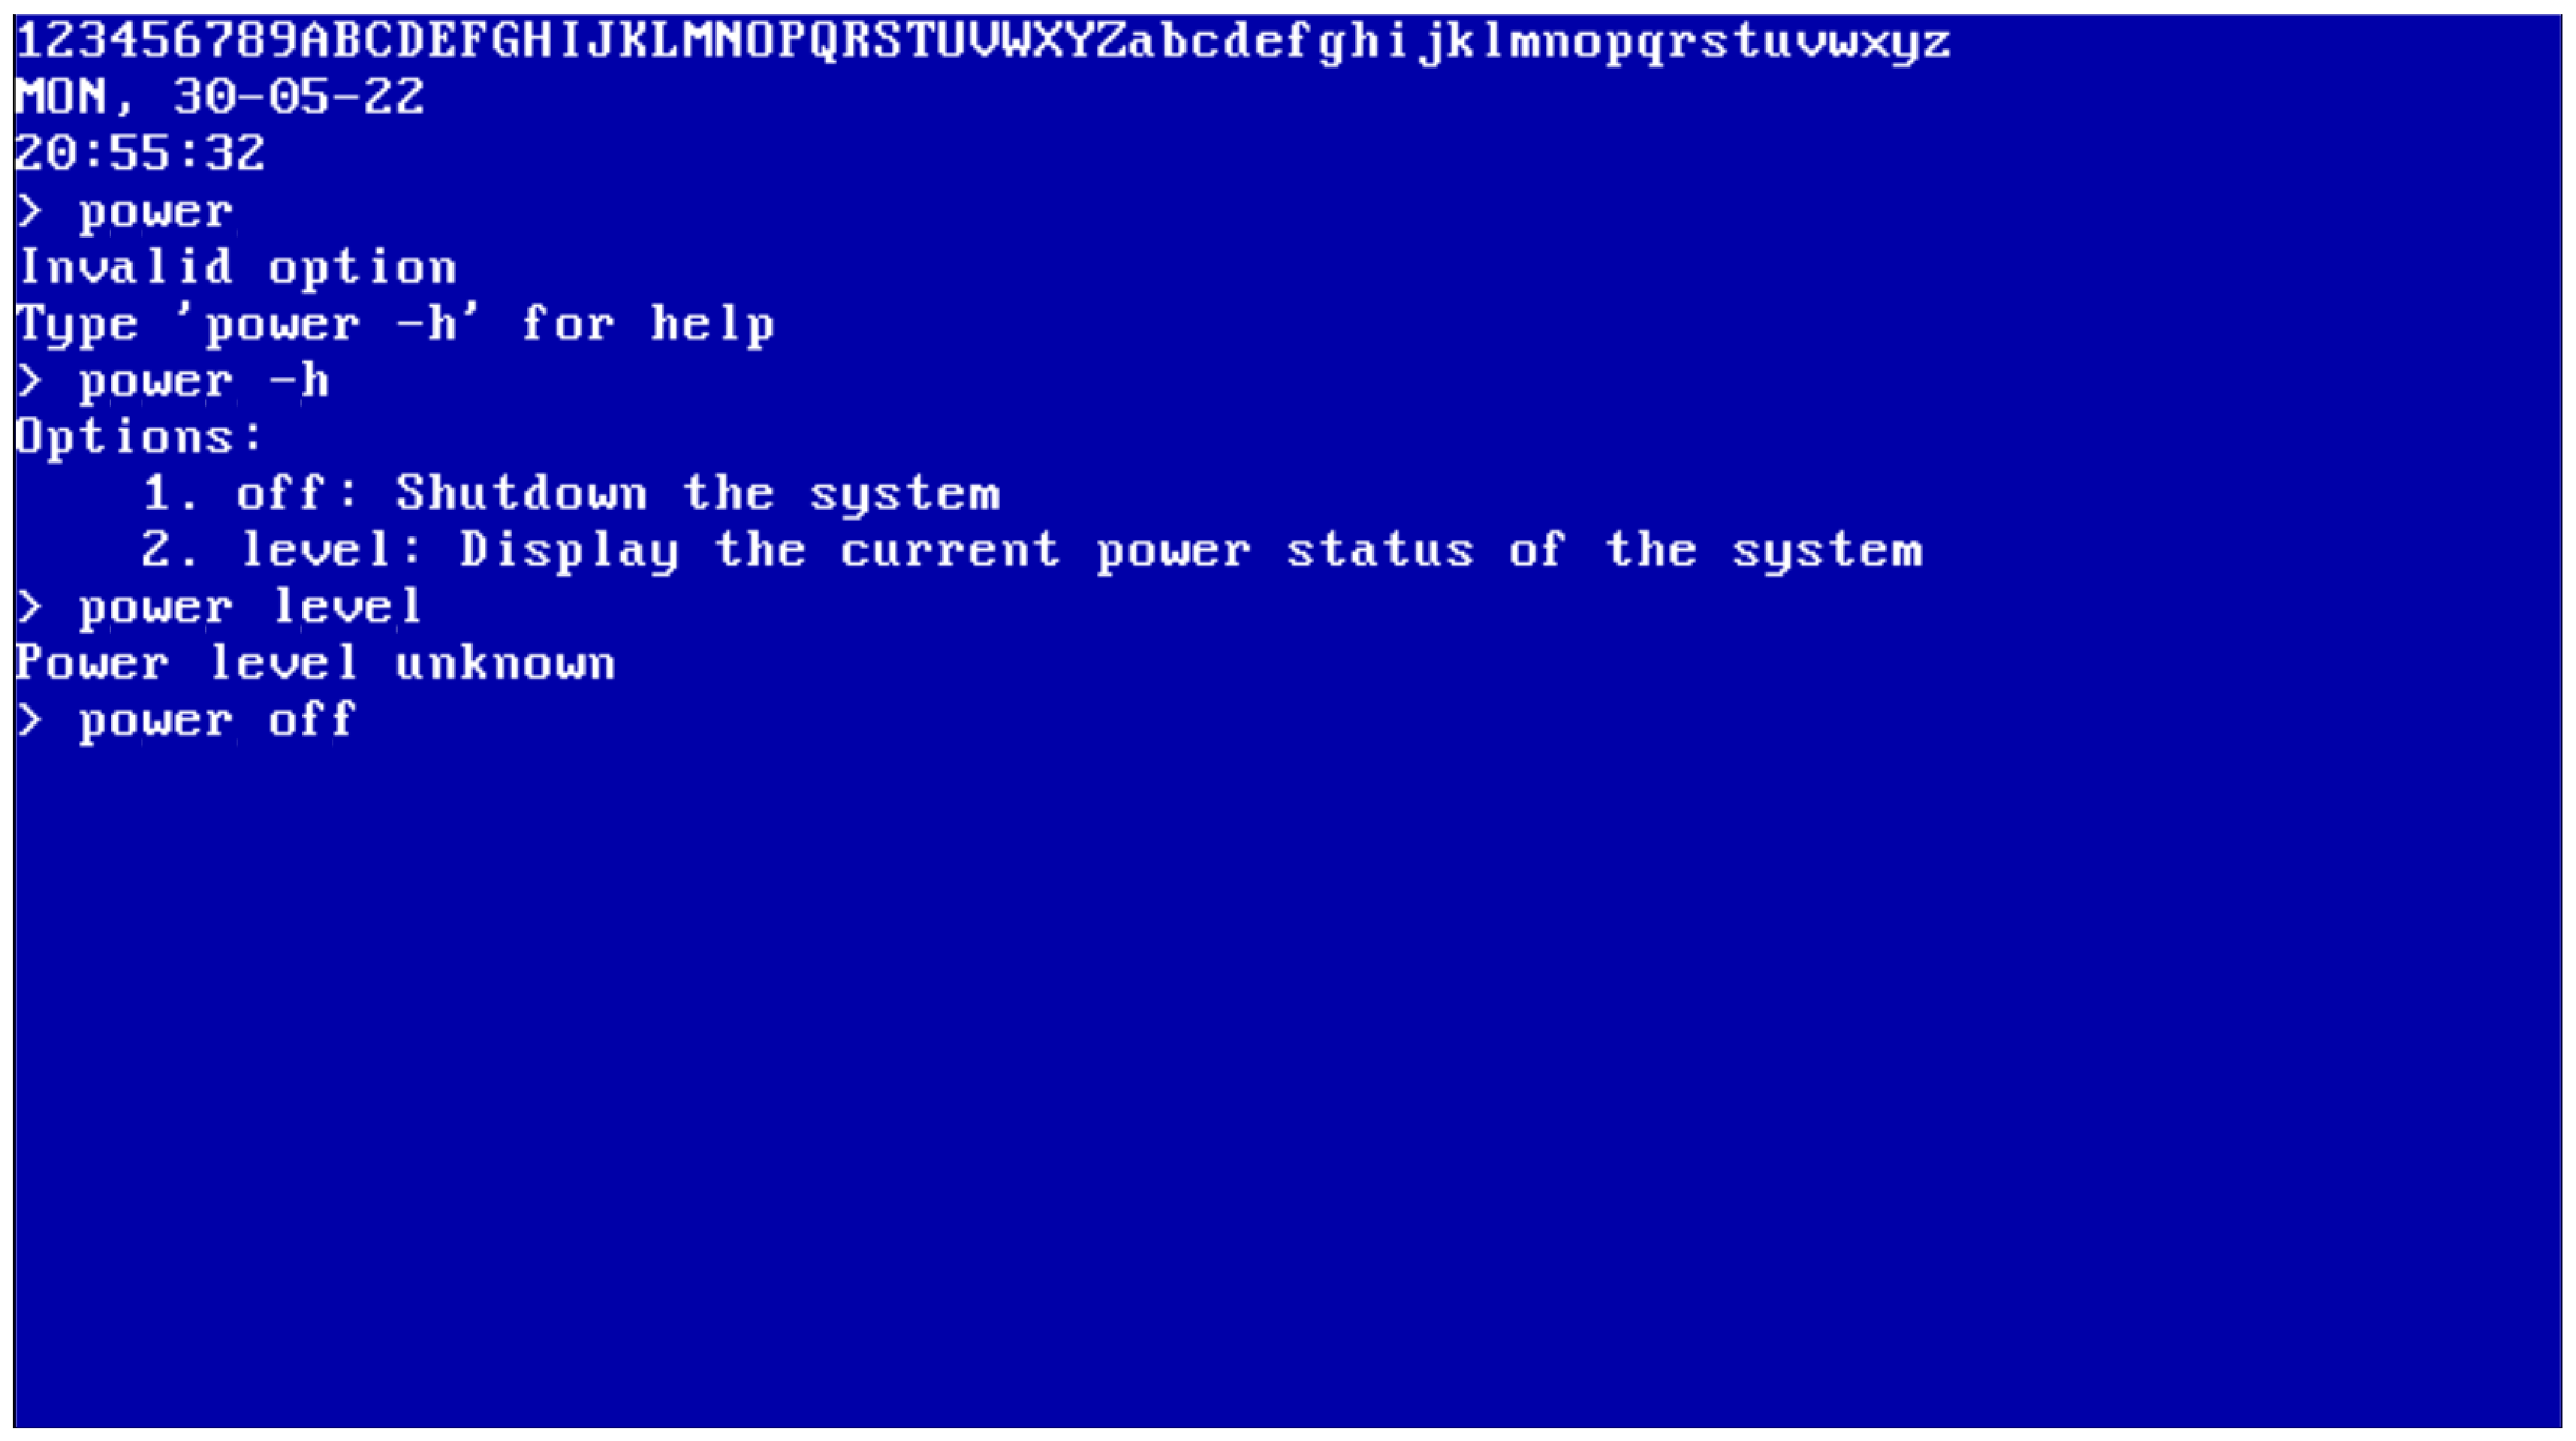
\includegraphics[scale=0.25]{figures/powercom.eps}
  \caption{Using \texttt{power} command}
\label{fig:powercom}
\end{figure}

\section{Using the Editor}
The line editor is ran from the shell by using the \texttt{edit} command. The address of the buffer should be passed as an argument. If the buffer is empty, then the total number of bytes is shown to be zero. Files are edited and their contents are listed using \texttt{*edit} and \texttt{*list} commands, respectively. Note that \texttt{*list} command clears the screen and then displays the contents of the buffer. To exit the editor, \texttt{*exit} command is used. Contents of the buffer are written to the disk using \texttt{disk write} command. \autoref{fig:editor1} shows these commands in action.\\
The same sectors of the disk to which we have written earlier can be read again and opened and listed in the editor. \autoref{fig:editor2} is a proof that the line editor and disk read/write commands are able to successfully able to create, save and edit files.
\begin{figure}[H]
  \begin{subfigure}{.5\textwidth}
  \centering
  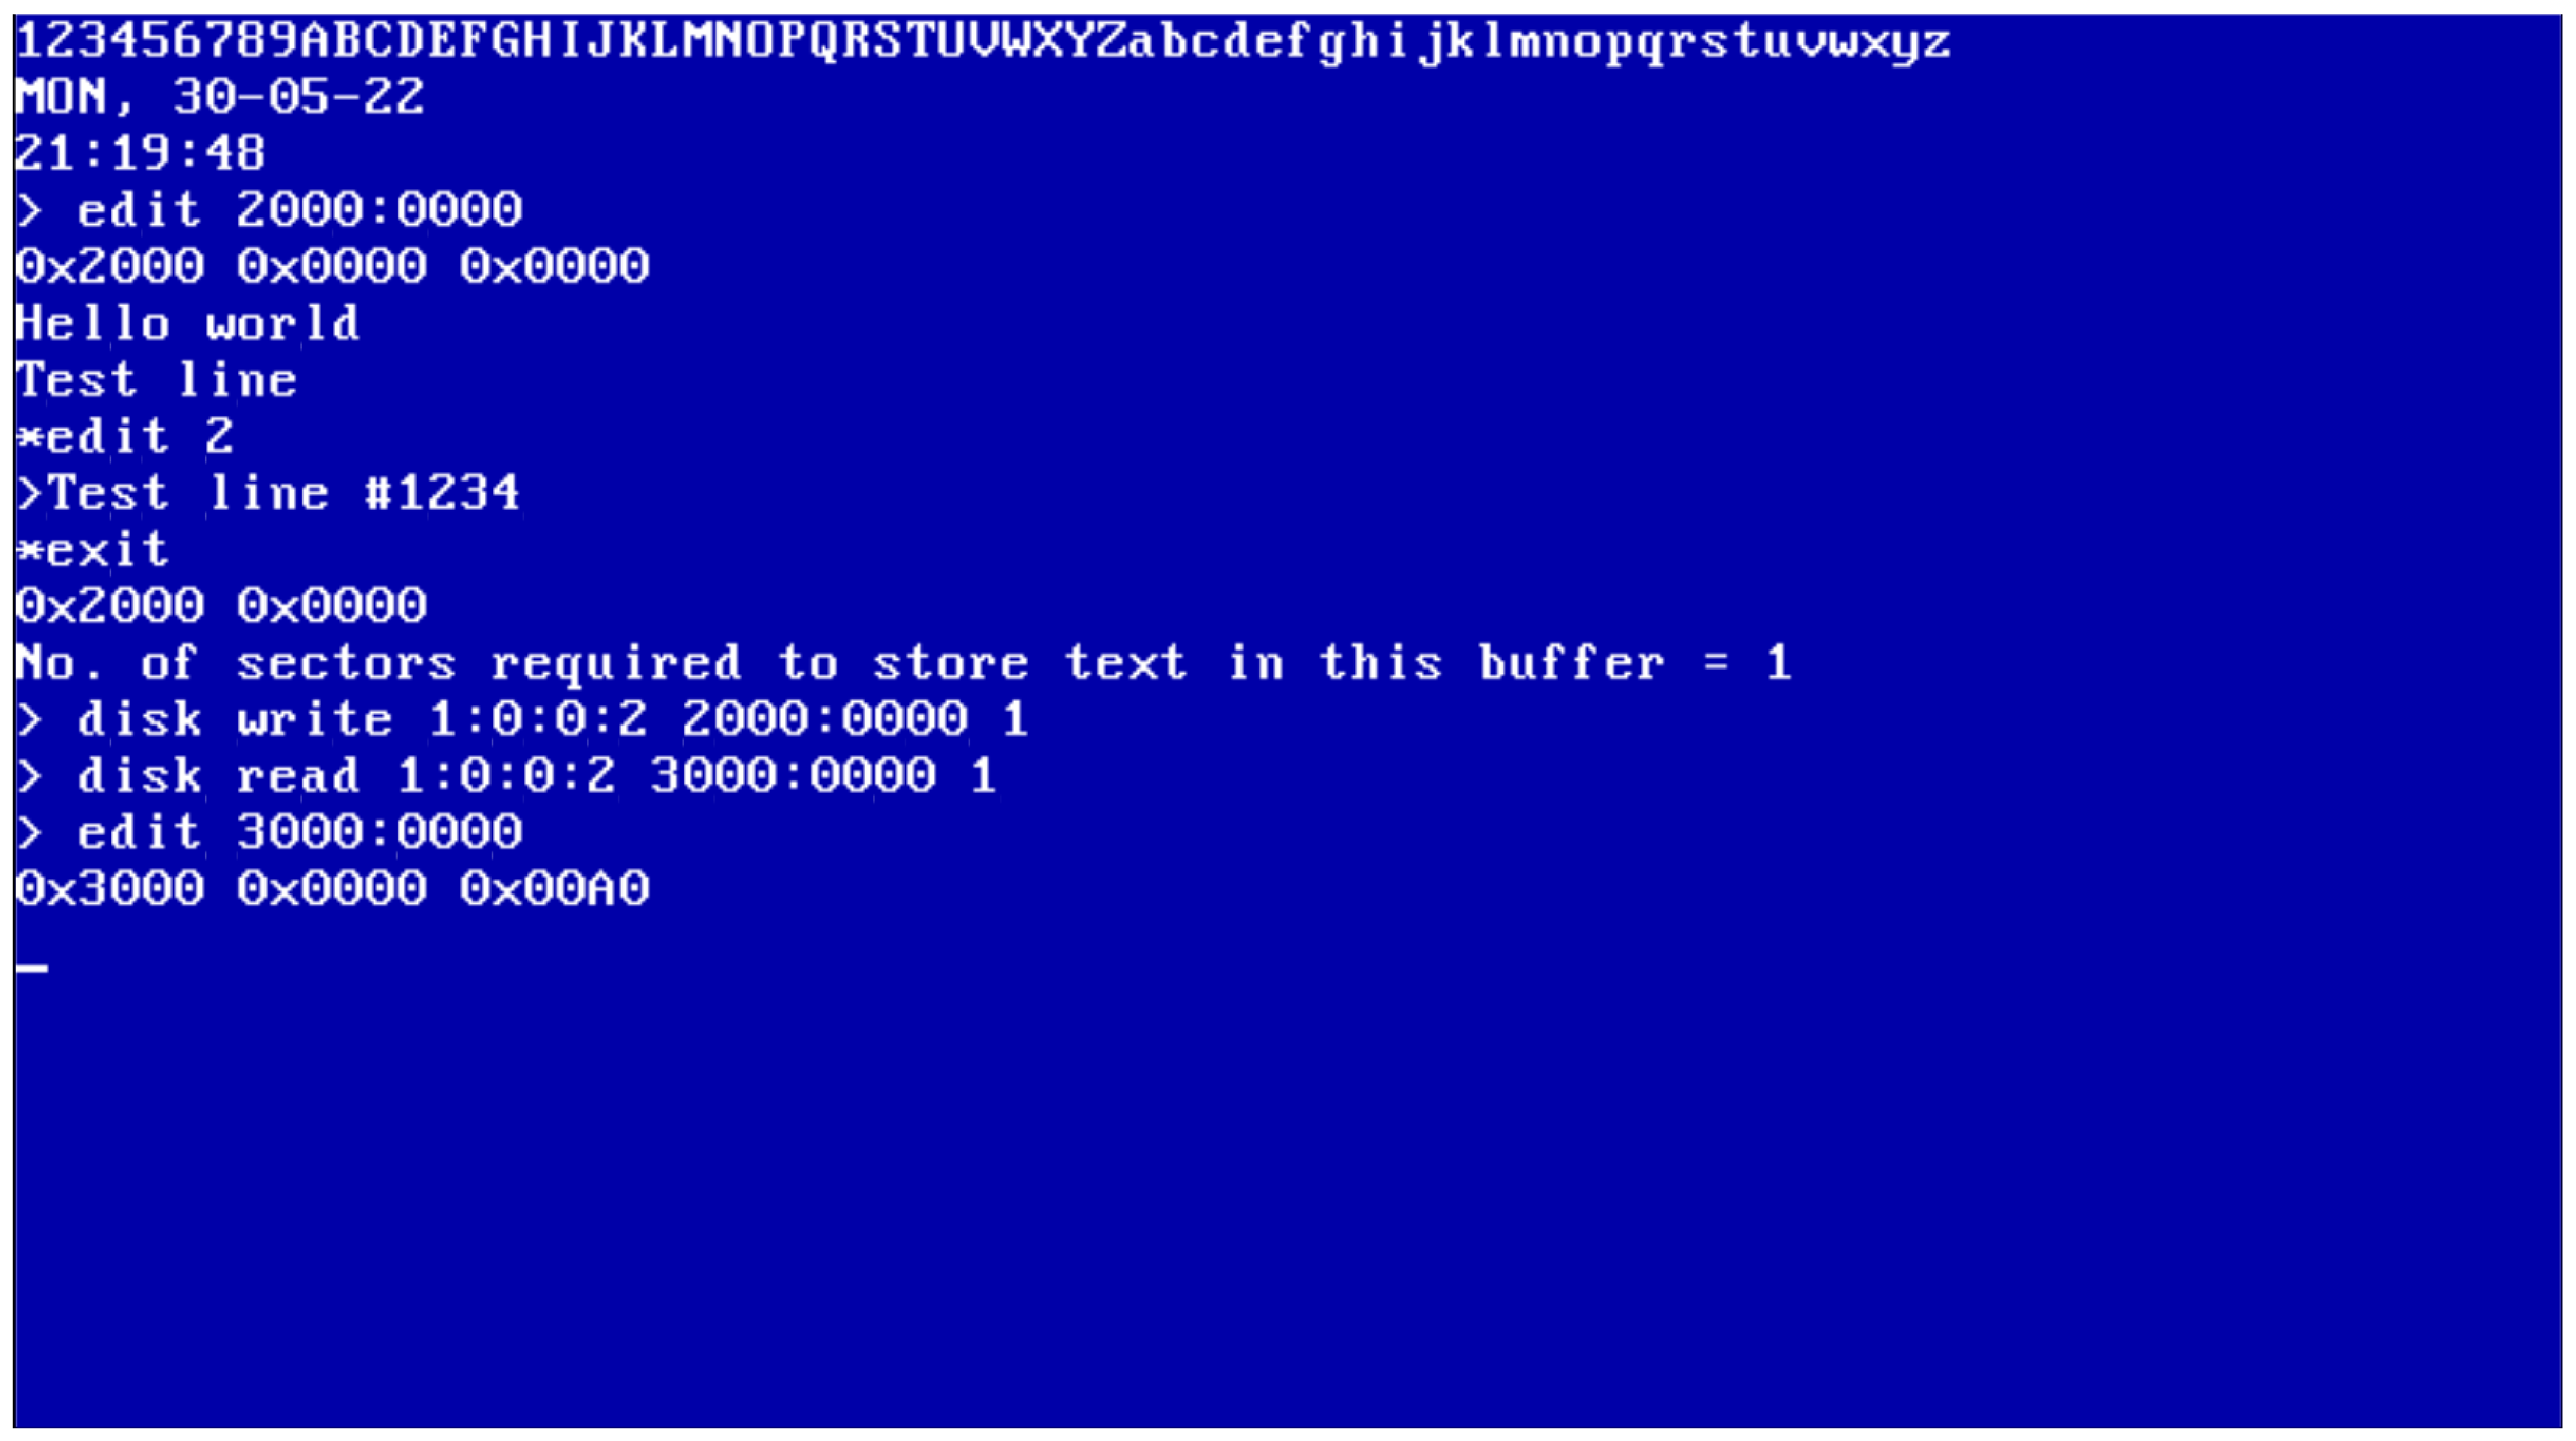
\includegraphics[scale=0.13]{figures/editor1.eps}
  \caption{Saving a new file to disk}
  \label{fig:editor1}
  \end{subfigure}
  \begin{subfigure}{.5\textwidth}
  \centering
  
\includegraphics[scale=0.13]{figures/editor2.eps}
  \caption{Successful operation of \texttt{edit} and \texttt{disk}}
  \label{fig:editor2}  
  \end{subfigure}
\caption{Using \texttt{edit} to create and edit a file}
\end{figure}

\section{Bugs}
The project has only three known bugs which is astonishing because it has been completely written in assembly language. These bugs are:
\begin{enumerate}
  \item \texttt{power level} command is not able to show the charge in the battery of the machine on which the emulator is running. This is shown in \autoref{fig:powercom}.
  \item Executing an invalid command string in the line editor insert that command string except for the asterisk. This is shown in \autoref{fig:faultycomm}.
  \item System might become unstable if an intersegment call is performed.
\end{enumerate}
\begin{figure}[H]
  \begin{subfigure}{.5\textwidth}
  \centering
  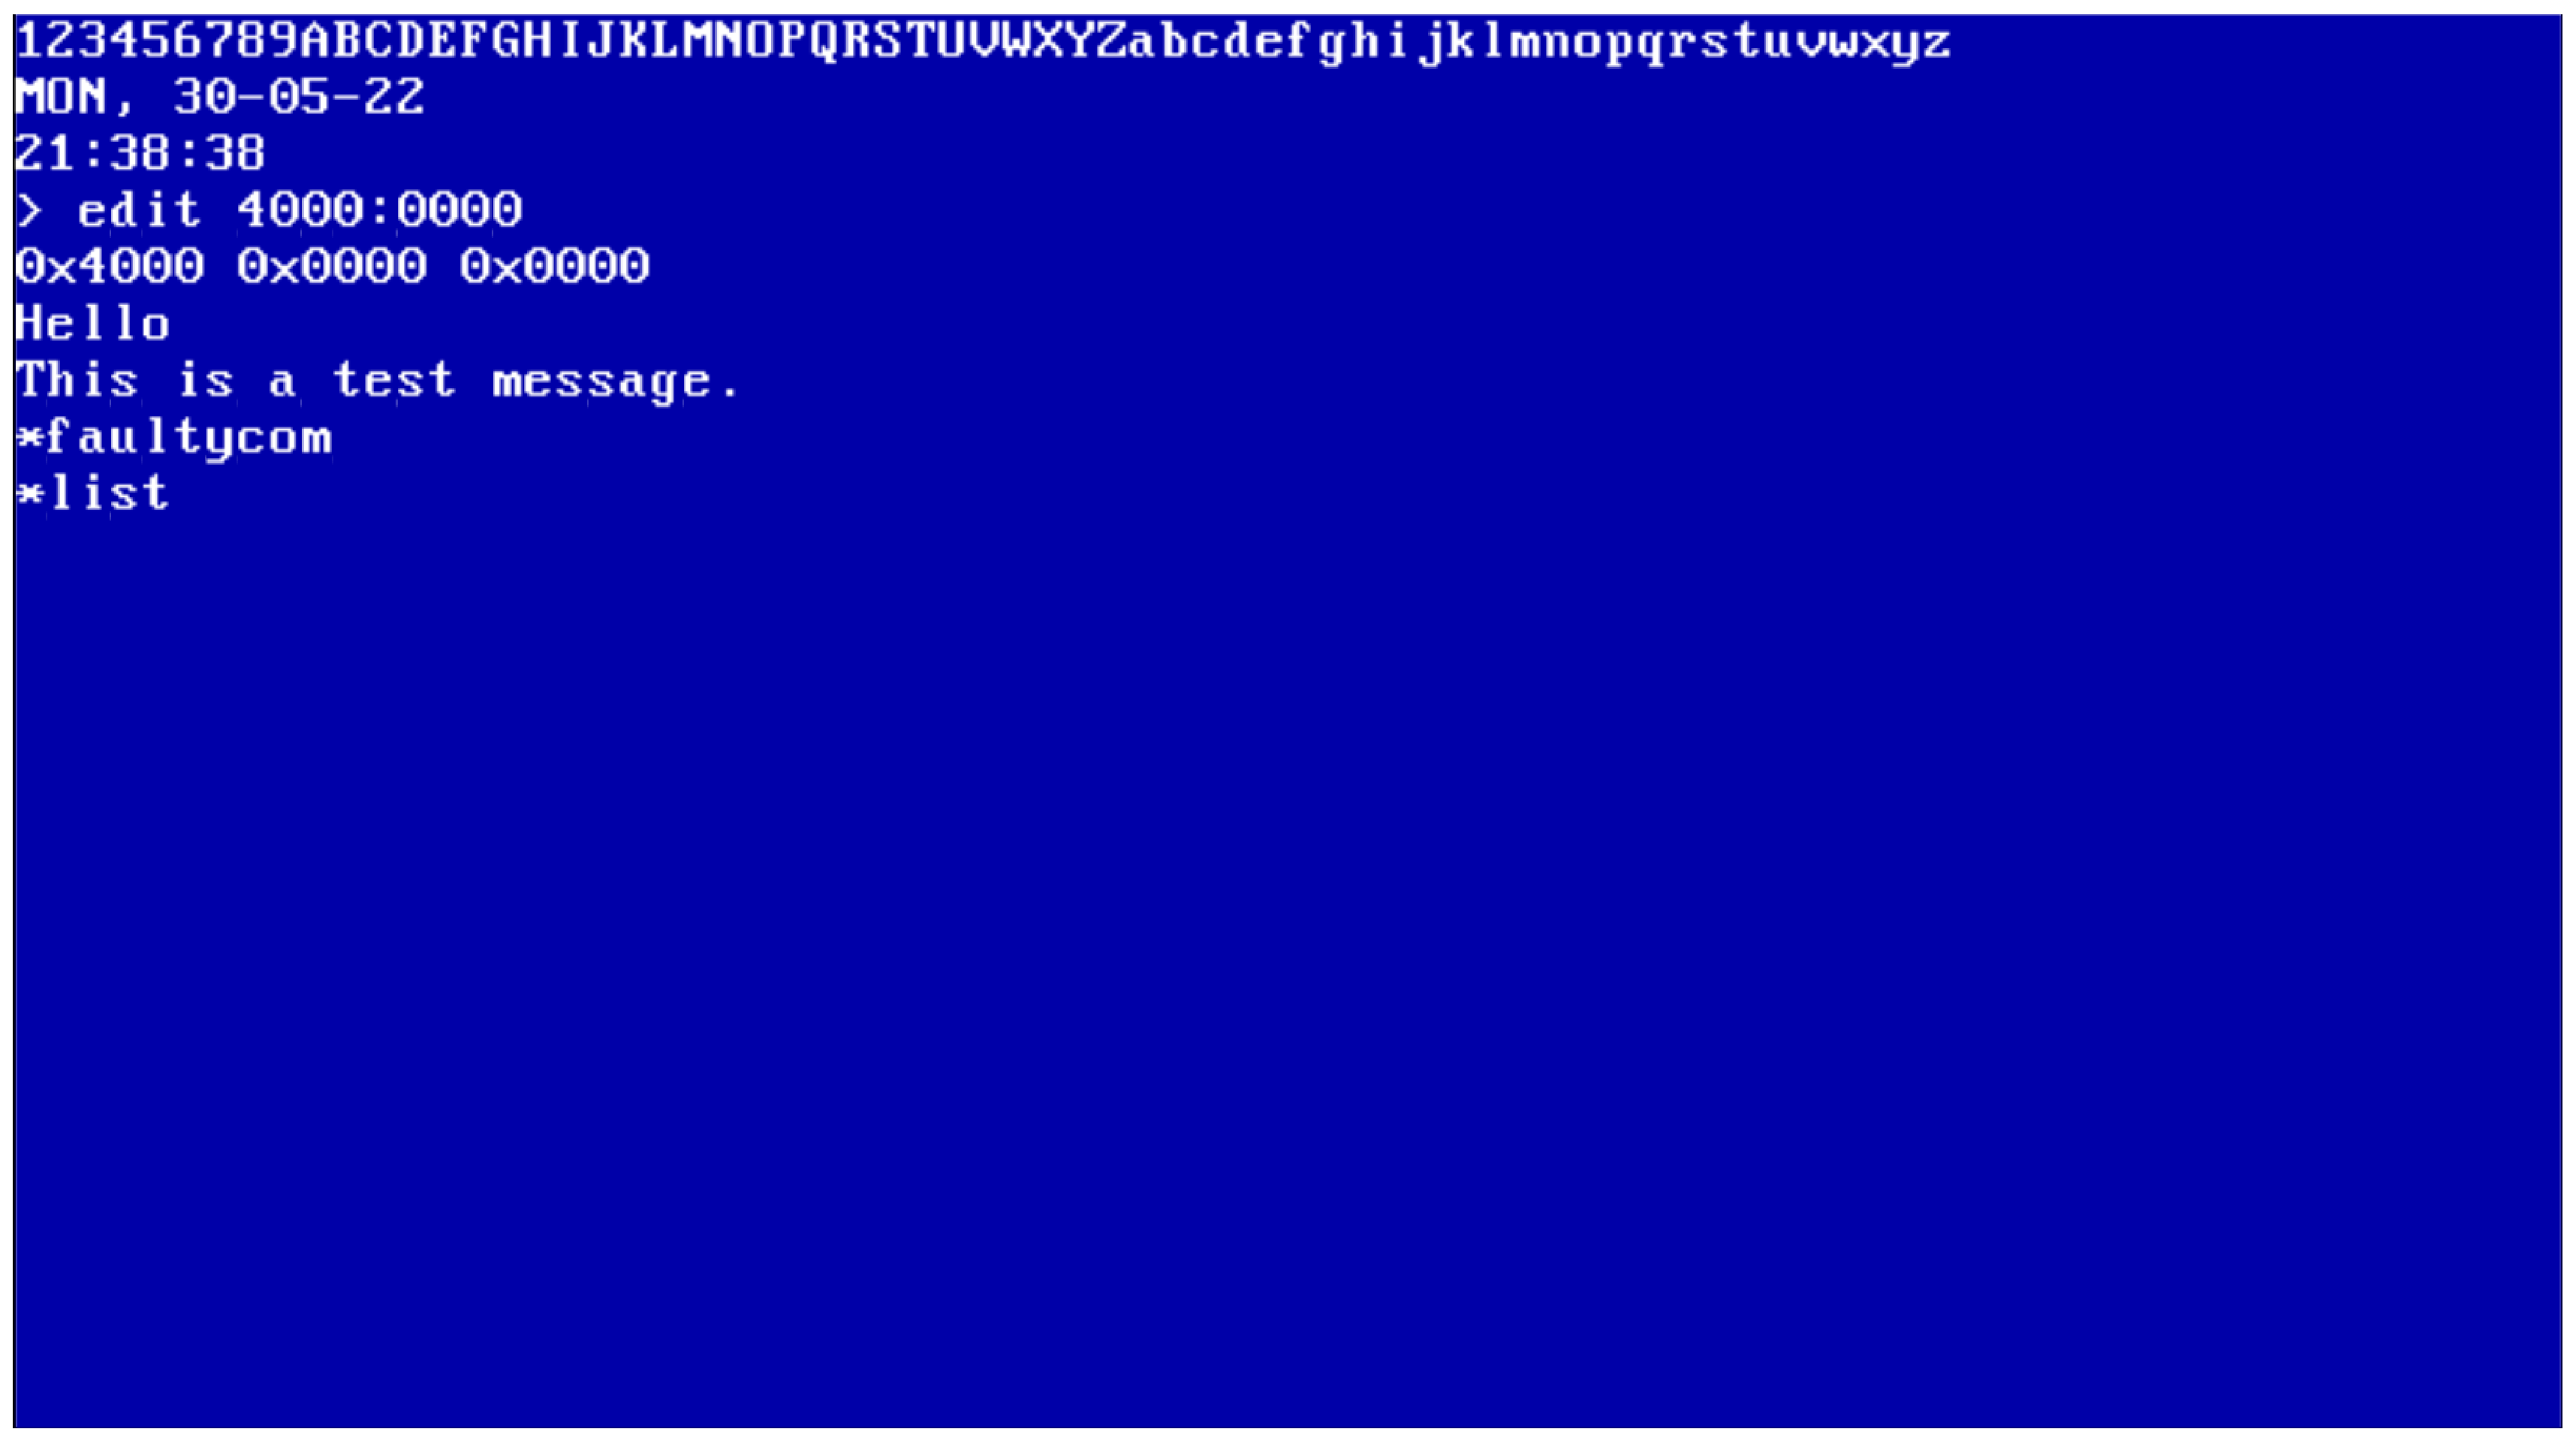
\includegraphics[scale=0.13]{figures/faultycomm1.eps}
  \caption{Entering an invalid command in the editor}
  \label{fig:faultycomm1}
  \end{subfigure}
  \begin{subfigure}{.5\textwidth}
  \centering
  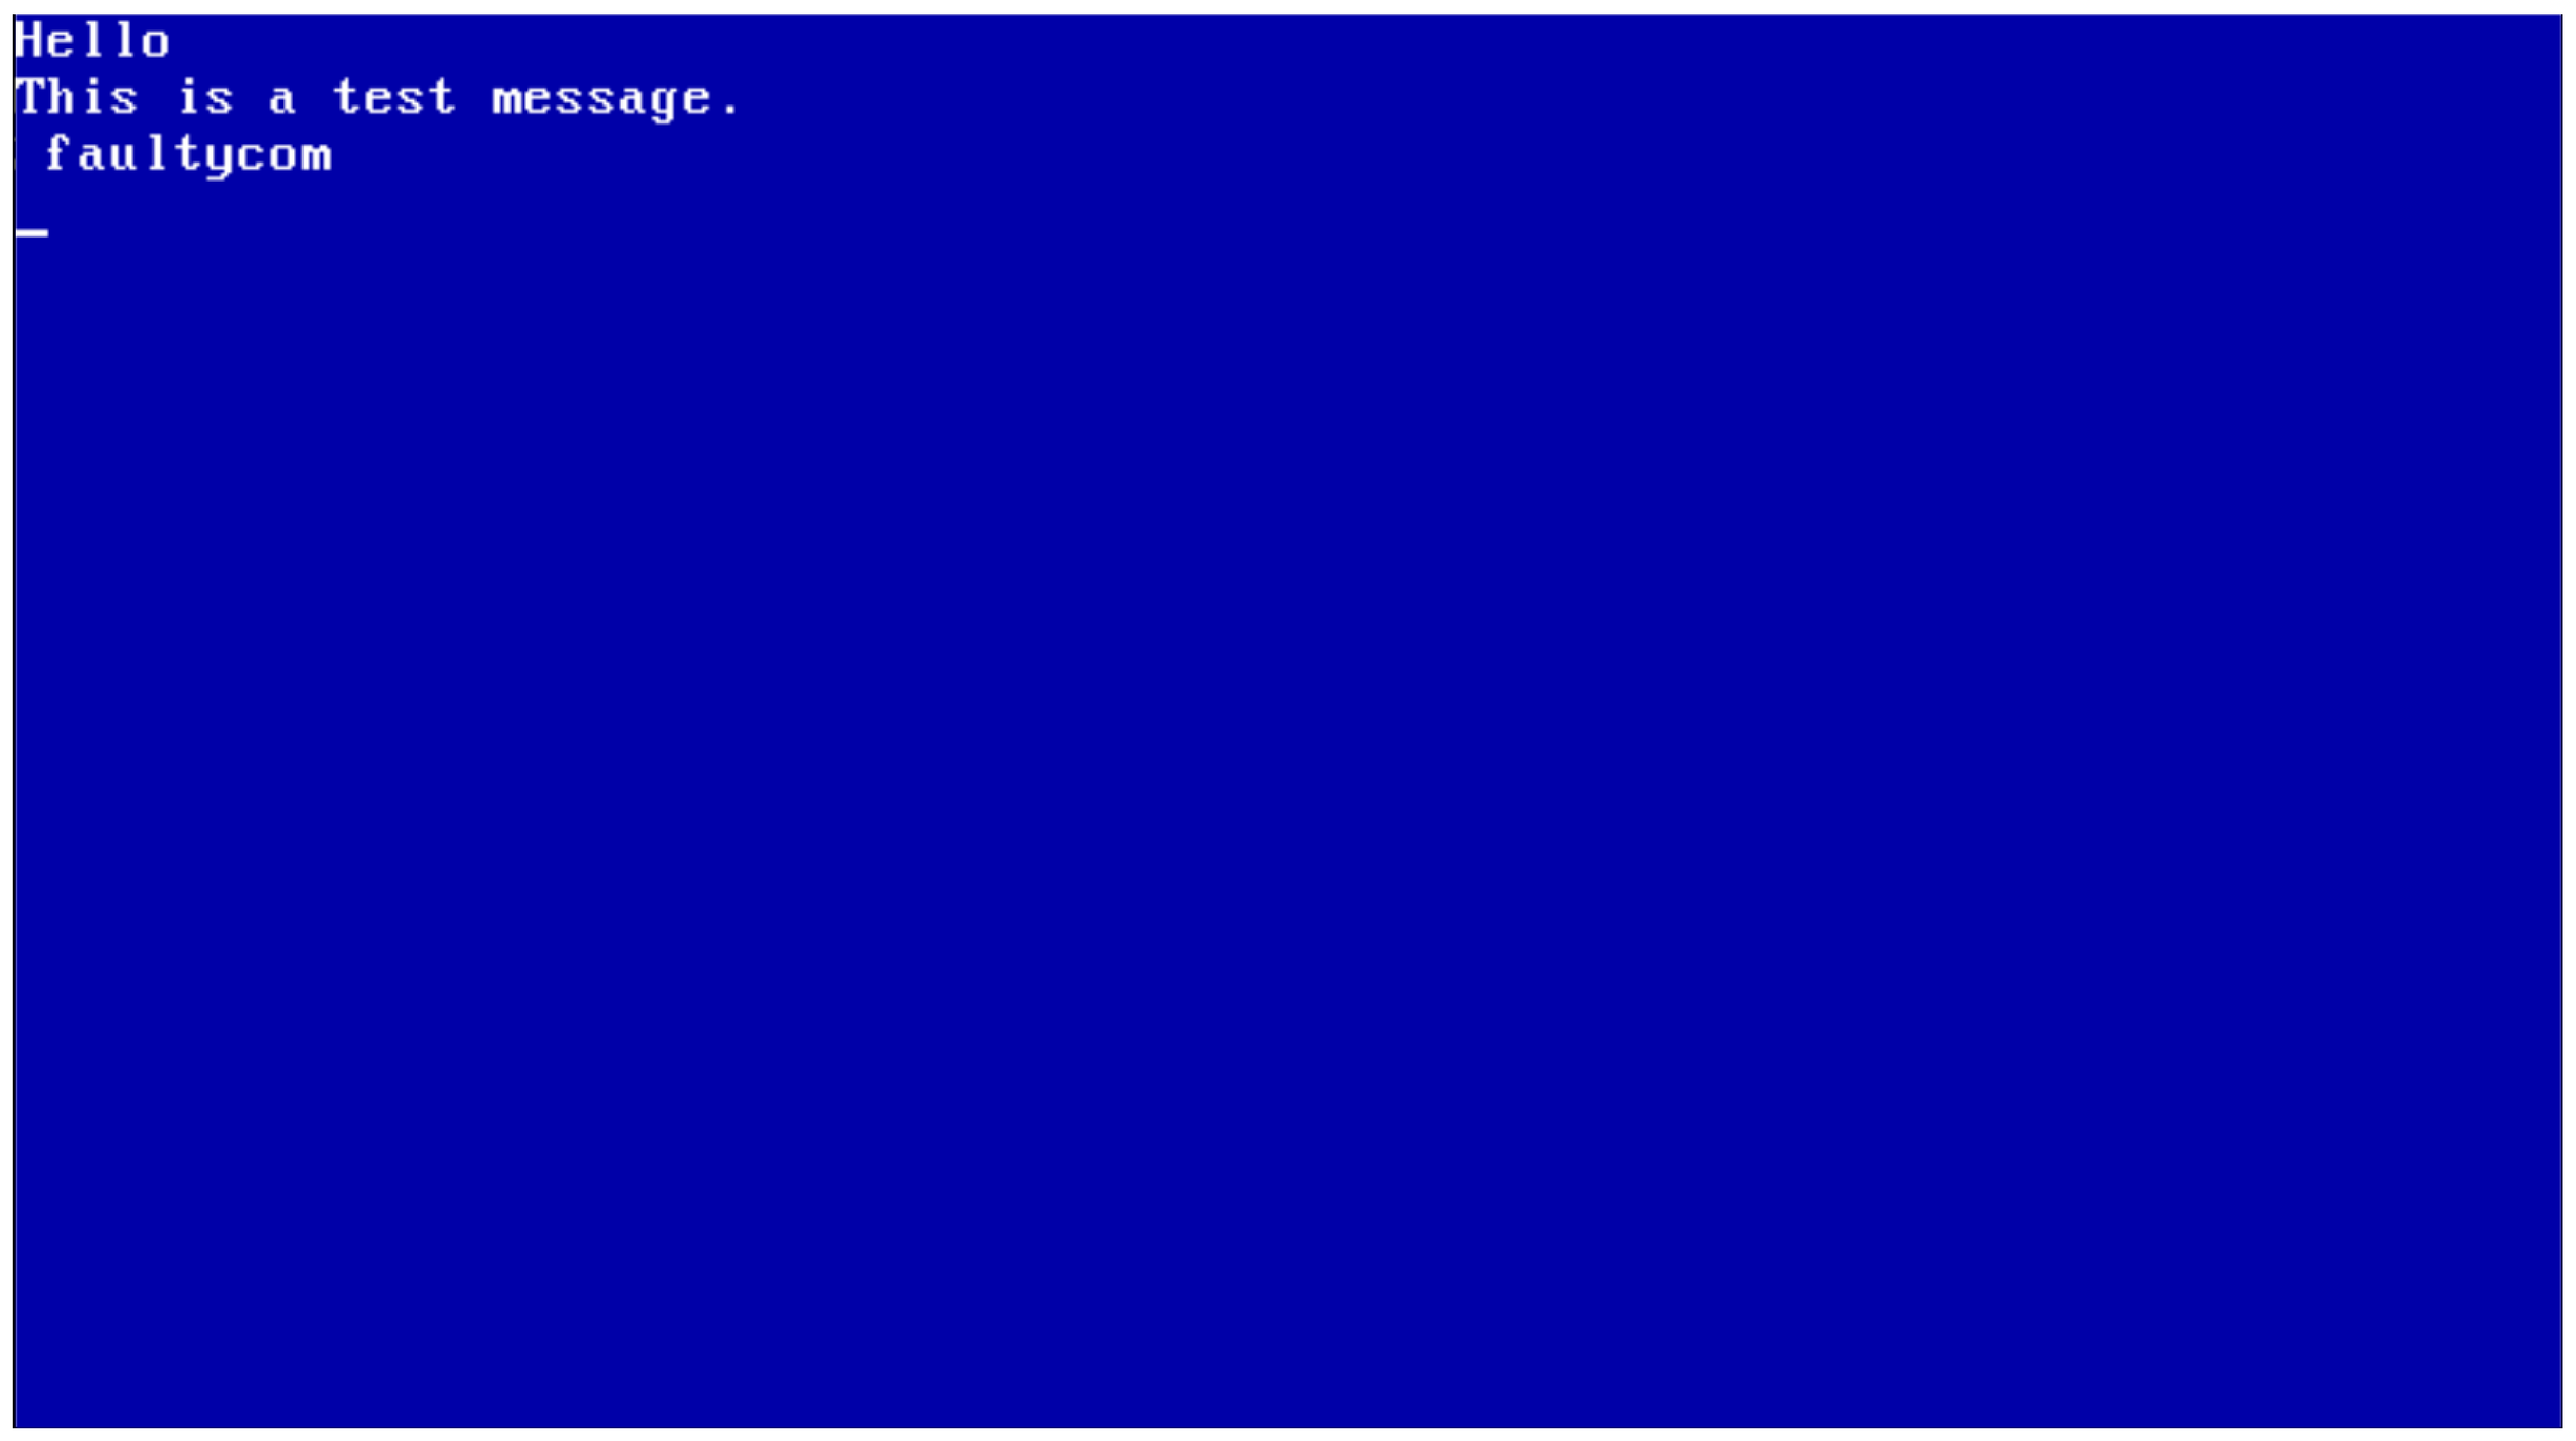
\includegraphics[scale=0.13]{figures/faultycomm2.eps}
  \caption{Listing of the file reveals the bug}
  \label{fig:faultycomm2}  
  \end{subfigure}
\caption{Bug in line editor causing it include contents of invalid commands}
\label{fig:faultycomm}
\end{figure}

\section{Discussion}
CrazyOS is comparable to disk operating systems (DOS) like CP/M and MS-DOS v1.25. Both MS-DOS v1.25 and CrazyOS have many similarities, few of which are:
\begin{enumerate}
  \item Both operating systems work in real mode.
  \item The command-prompt/shell of both of these operating system has commands built into the source code of the shell itself.
  \item Both operating systems make use of BIOS calls to access the hardware.
  \item Both of these operating system are meant for a single user only.
  \item Neither CrazyOS nor MS-DOS v1.25 has the ability to multitask between different software. 
\end{enumerate}
However, unlike MS-DOS, CrazyOS
\begin{enumerate}
  \item does not have any system calls which makes it heavily dependent on the BIOS calls provided by the OEM.
  \item does not support running applications having binary size greater than 64 kiB. Returning to shell from smaller applications after an intersegment call makes the shell unstable.
  \item does not use proper file allocation table (FAT). Therefore, disk space is not utilized efficiently.
\end{enumerate}
All modern day operating systems, like Linux kernel based distros and Windows 10, are far superior than DOS. They are one of the most complex pieces of software in the world which provide programmers and everyday users with hardware support, system calls, and file systems among many other things which allow them to use the resources of the machine efficiently and get their job done. With millions of lines of codes, even tech-gurus can only master a few integral components of the operating system in their lifetime. Clearly, the simplicity of CrazyOS comes at the cost of functionality and makes it a toy operating system which can be used for educational purposes. Porting CrazyOS for x86-64 and ARM based processors while implementing a few fundamental system calls and a file system will tremendously improve its usefulness.









